\section{Assinatura digital}

\begin{frame}[allowframebreaks]
\frametitle{Assinatura digital}
Uma assinatura digital é utilizada para validar a autenticidade e integridade de uma mensagem.

\vspace{3ex}
A base para assinaturas digitais é a criptografia assimétrica (utilizando chave pública e privada).
Exemplo: algoritmo RSA (Rivest-Shamir-Adleman).

\vspace{3ex}
Calcula-se o hash de um documento e encripta o hash (junto com outras informações) usando a chave privada. 

\vspace{3ex} 
O hash é rápido de se calcular e possui tamanho fixo.

\begin{figure}[h]
\centering
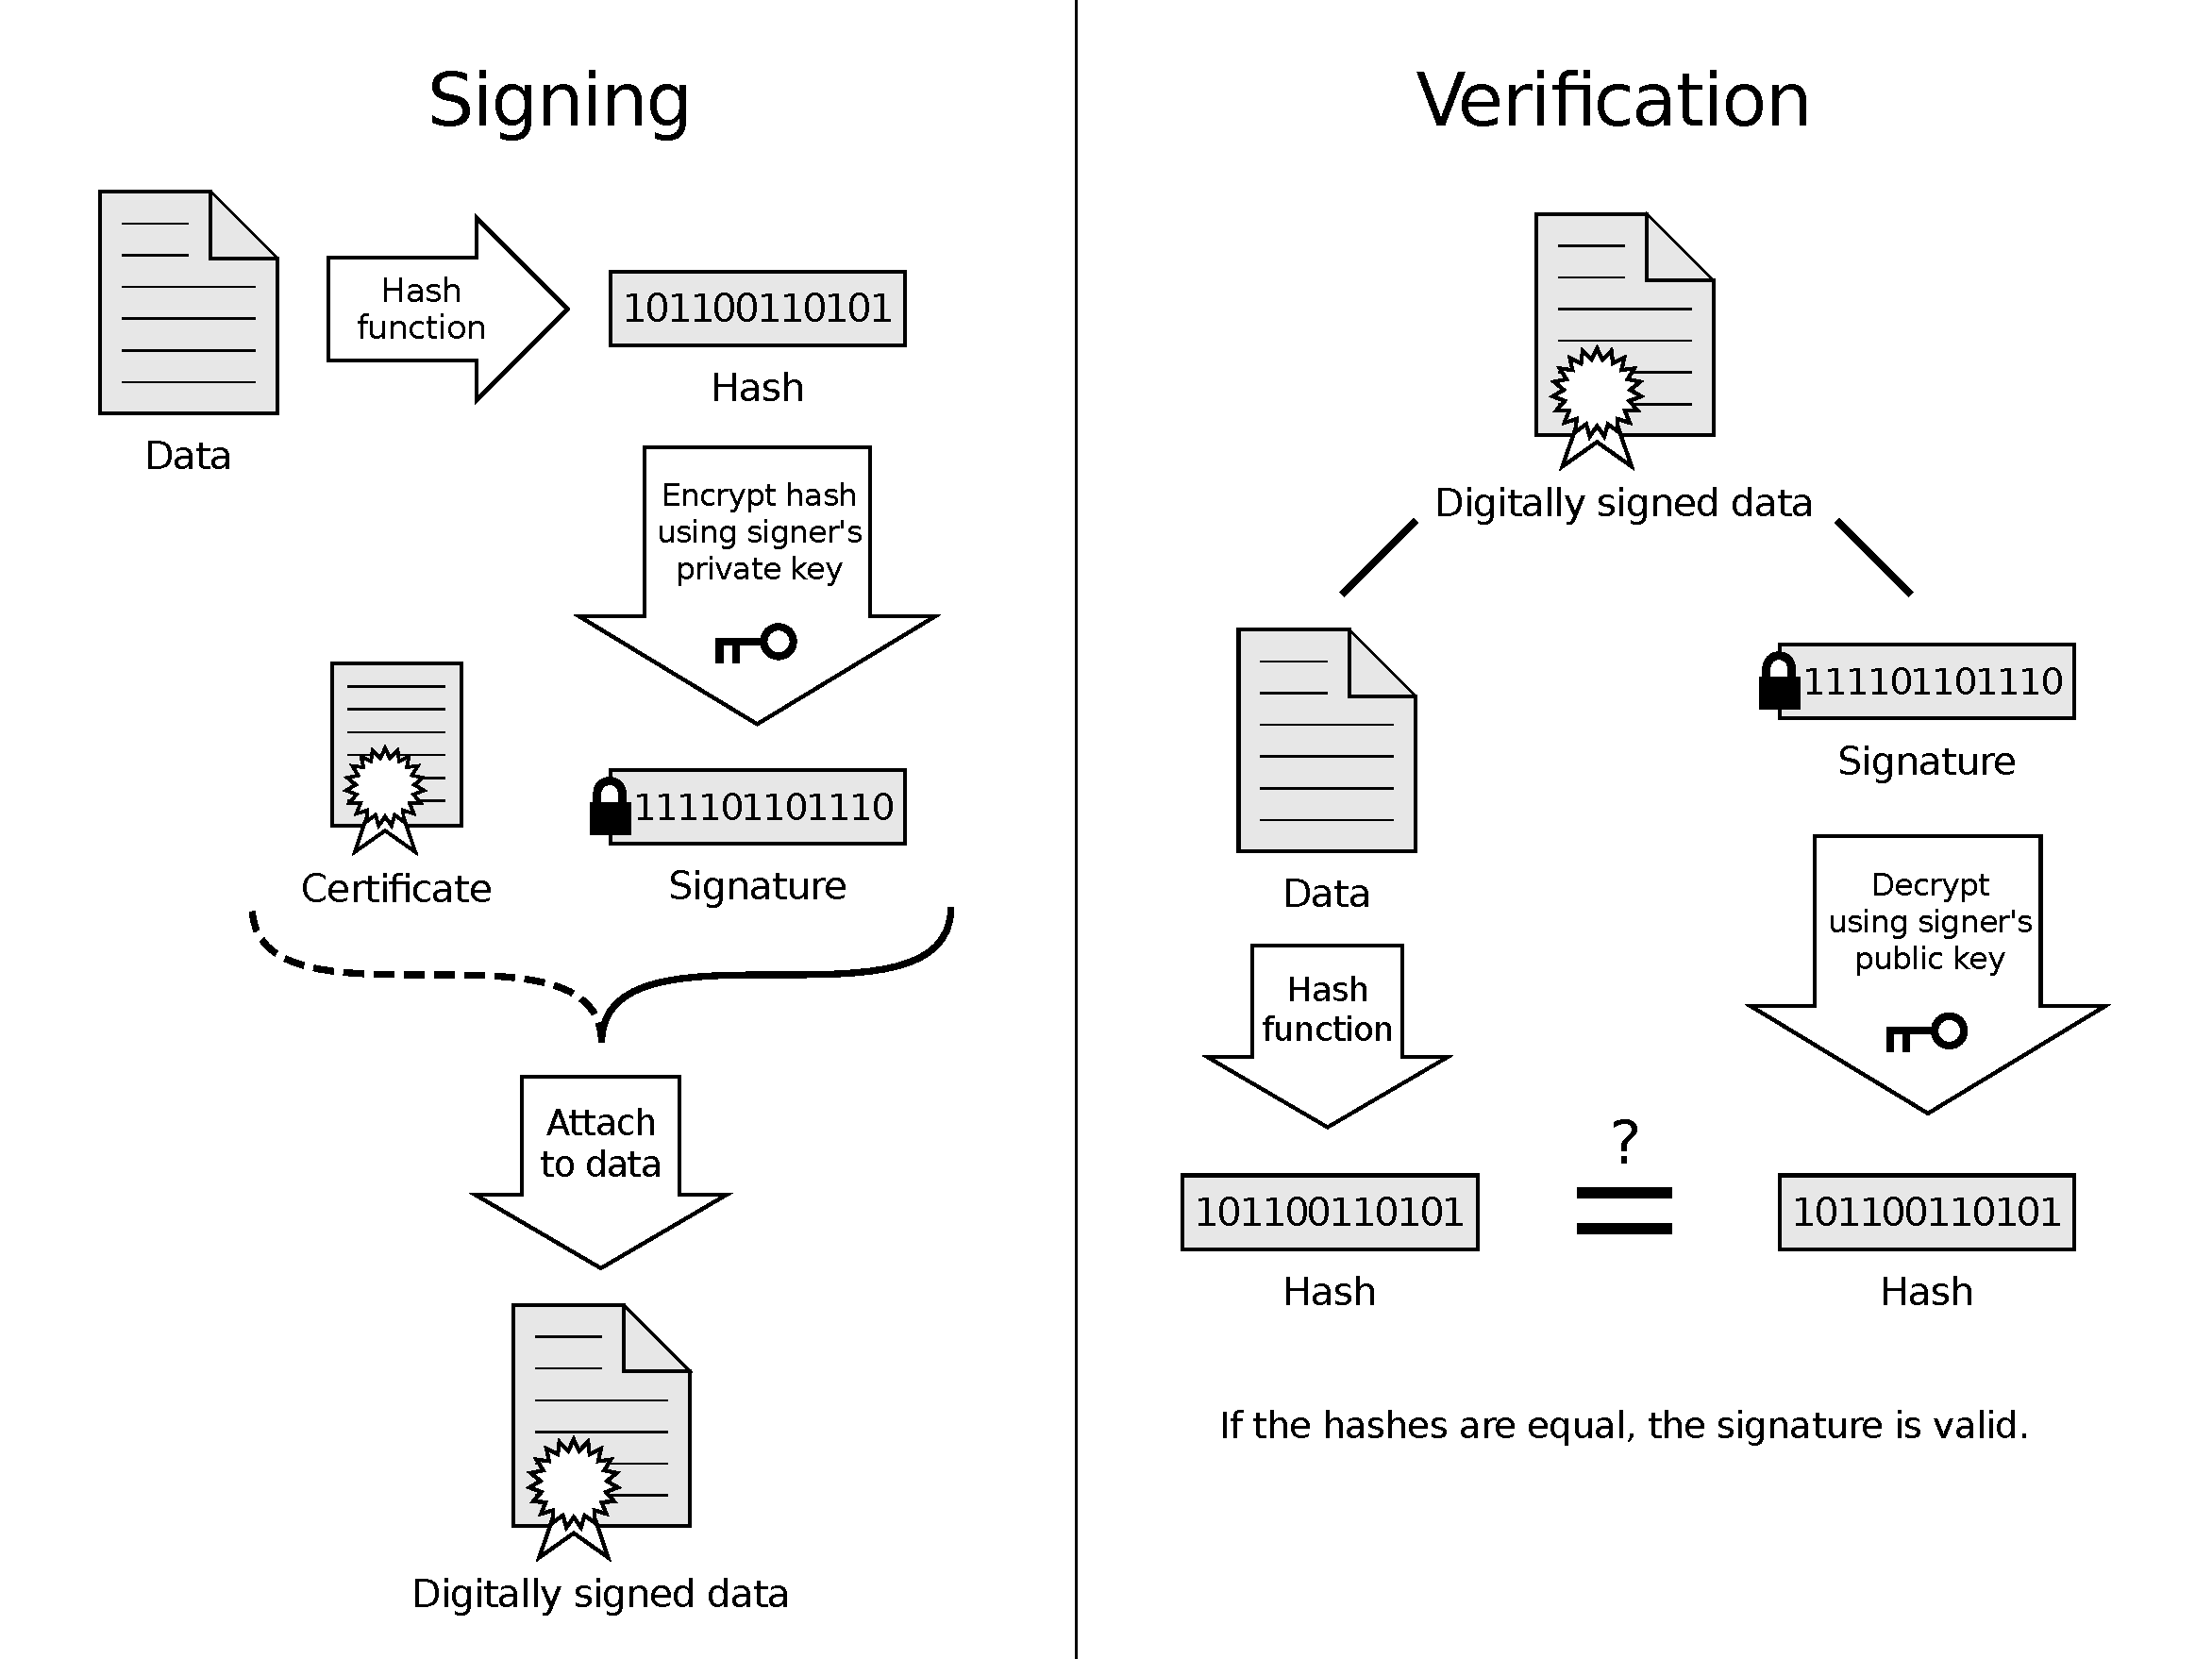
\includegraphics[width=0.8\textwidth,height=0.8\textheight,keepaspectratio]{figures/digitalsignaturediagram.pdf}
\caption{Diagrama de assinatura digital de documentos (\url{https://commons.wikimedia.org/wiki/File:Digital_Signature_diagram.svg}).}
\label{fig-digi-sign}
\end{figure}

Certificado digital \textbf{x} assinatura digital\\
O certificado digital é uma documento digital emitido por uma autoridade de certificação (CA). 
As CAs agem como terceiros confiáveis aceitando, autenticando, emitindo e mantendo certificados digitais. 
O certificado digital faz a ligação entre a chave pública e a identidade de um agente, permitindo
verificar se determinada chave pertence a tal pessoa ou entidade.

\end{frame}



\begin{frame}
\frametitle{Criptografia}

\begin{itemize}
\item estenografia - ocultar uma mensagem dentro de outra
\item escrita oculta
\item criptografia - escrita segura
\end{itemize}

\end{frame}



\begin{frame}[allowframebreaks]
\frametitle{Estenografia}
\begin{figure}[h]
\centering
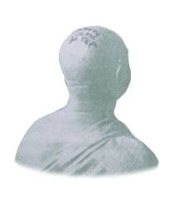
\includegraphics[width=0.33\textwidth,height=0.7\textheight,keepaspectratio]{figures/herodotus.jpg}
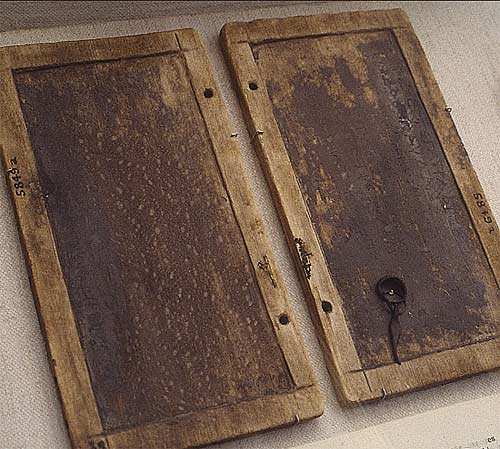
\includegraphics[width=0.33\textwidth,height=0.7\textheight,keepaspectratio]{figures/waxtablet.jpg}
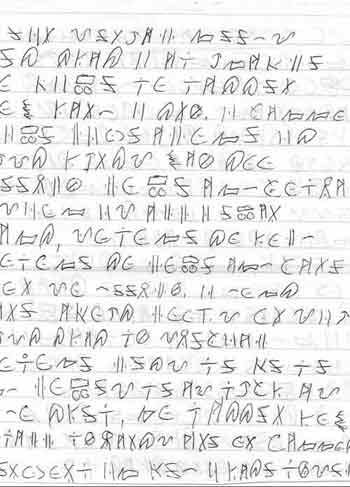
\includegraphics[width=0.33\textwidth,height=0.7\textheight,keepaspectratio]{figures/gangcode.jpg}
\caption{Tatuagem de Heródoto. Tábuas de cera. Código de gangues.}
\label{fig-estenografia}
\end{figure}

\begin{itemize}
\item tinta invisível
\item micropontos
\item bits de menor valor
\end{itemize}
\end{frame}




\begin{frame}
\frametitle{Cifra de transposição}

A Cítala é um ferramenta de criptografia utilizada pelos gregos antigos e espartanos para envio de mensagens secretas
durante as campanhas militares.
\begin{figure}[h]
\centering
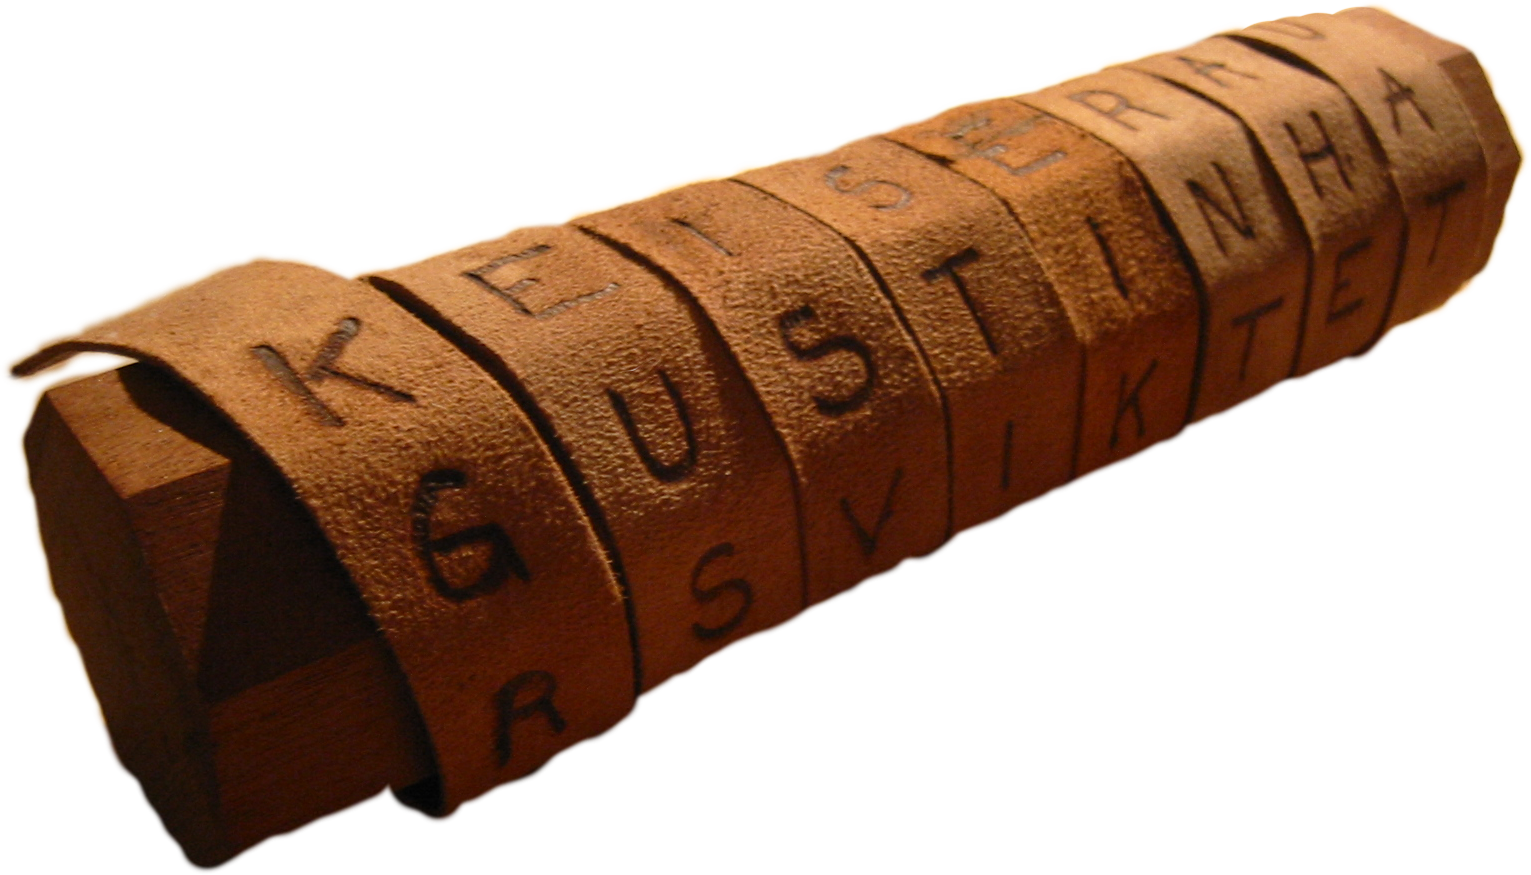
\includegraphics[width=0.6\textwidth,height=0.5\textheight,keepaspectratio]{figures/cifratransposicao.png}
\caption{Cítala (ou bastão de Licurgo). Cifra de transposição. \url{https://en.wikipedia.org/wiki/Scytale}}
\label{fig-cifratrans}
\end{figure}
\end{frame}


\begin{frame}[allowframebreaks]
\frametitle{Cifra de César}

\begin{figure}[h]
\centering
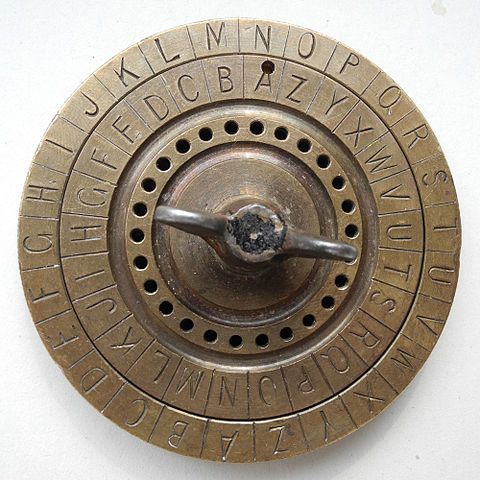
\includegraphics[width=0.5\textwidth,height=0.5\textheight,keepaspectratio]{figures/caesar.jpg}
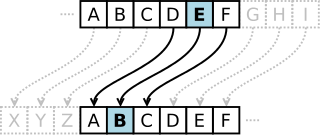
\includegraphics[width=0.5\textwidth,height=0.5\textheight,keepaspectratio]{figures/CaesarCipher.png}
\caption{Cifra de César. \url{https://en.wikipedia.org/wiki/Caesar_cipher}}
\label{fig-cifracaesar}
\end{figure}

ROT13 (\emph{rotate by 13 places}) é um caso específico da cífra de César com deslocamente de 13 posições, o que 
faz com que o algoritmo de codificação e decodificação seja o mesmo.
ROT13 era utilizado na década de 80 para esconder piadas potencialmente ofencivas, respostas de enigmas, ou 
outros \emph{spoilers}. É utilizado para esconder endereços de e-mails de \emph{spam bots}.
\url{https://en.wikipedia.org/wiki/ROT13}

\begin{figure}[h]
\centering
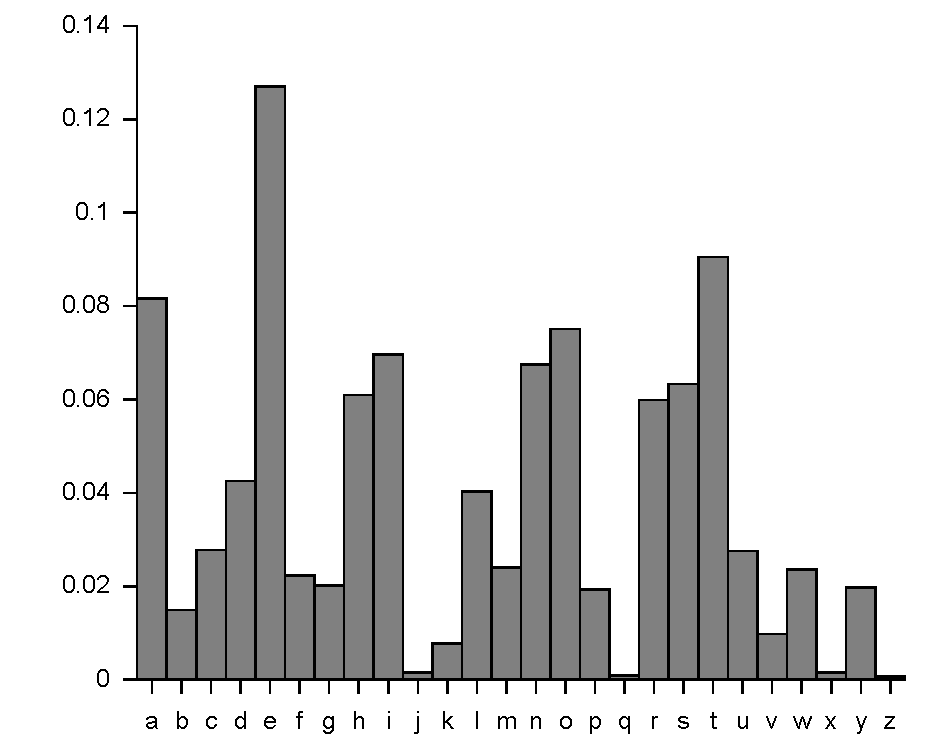
\includegraphics[width=0.5\textwidth,height=0.5\textheight,keepaspectratio]{figures/English_letter_frequency.pdf}
\caption{Distribuição de frequência dos caracteres no Inglês. \url{https://en.wikipedia.org/wiki/Caesar_cipher}}
\label{fig-eng-letters-dist}
\end{figure}

\end{frame}



\begin{frame}
\frametitle{Cifra de Beale}
Substitui cada palavra ou sequência por um código (utilizando uma referência, por exemplo, um livro).

\begin{figure}[h]
\centering
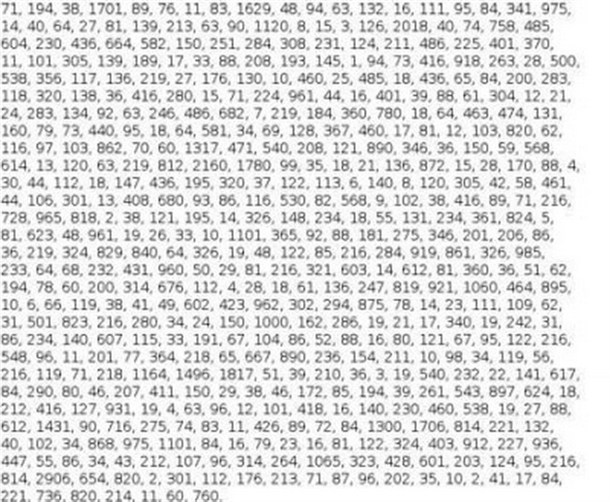
\includegraphics[width=0.7\textwidth,height=0.5\textheight,keepaspectratio]{figures/beale.jpg}
\caption{Cifra de Beale.}
\label{fig-beale}
\end{figure}

\end{frame}






\begin{frame}[allowframebreaks]
\frametitle{Zodíaco}

\begin{figure}[h]
\centering
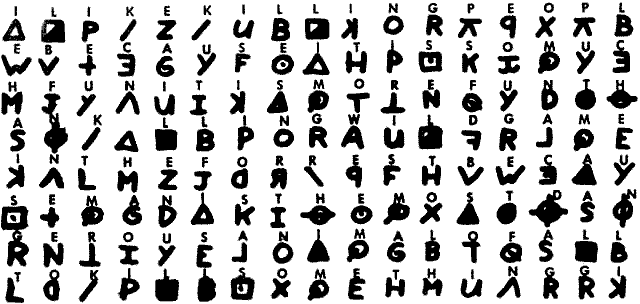
\includegraphics[width=0.5\textwidth,height=0.5\textheight,keepaspectratio]{figures/zodiaccipher.png}
\caption{Zodíaco. Múltiplos símbolos para caracteres comuns do alfabeto e anagramas.}
\label{fig-zodiac}
\end{figure}

O código foi quebrado apenas no final de 2020.\\
\fullcite{goodin_zodiac_2020}
\vspace{2ex}
\fullcite{bauer_zodiac_nodate}

\end{frame}


\begin{frame}
\frametitle{Vigenère Cipher}

Cifra polialfabética (cifra baseada na substituição, usando vários alfabetos de substituição).
Utiliza as letras da chave para selecionar a coluna e as letras da mensagem para selecionar a linha.

\begin{figure}[h]
\centering
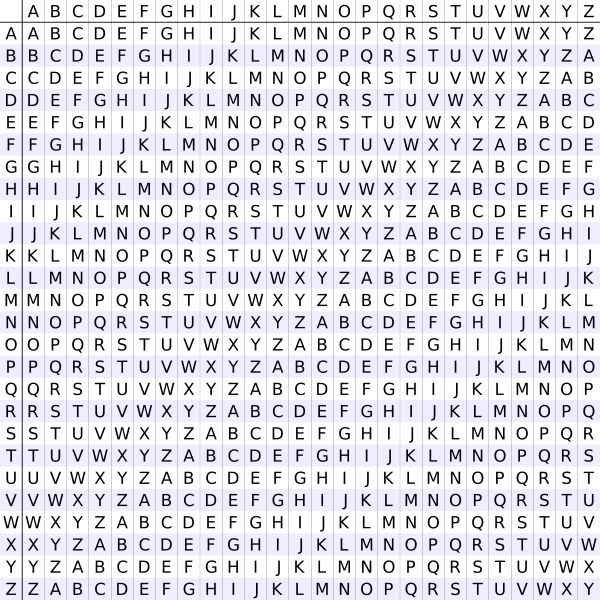
\includegraphics[width=0.8\textwidth,height=0.7\textheight,keepaspectratio]{figures/vigenere.png}
\caption{Cifra de Vigenère. Exemplo: mensagem ATTACKATDAWN, chave LEMONLEMONLE, texto cifrado LXFOPVEFRNHR.}
\label{fig-vigenere}
\end{figure}

\end{frame}


\begin{frame}
\frametitle{Cifras polialfabéticas baseadas em rotores}
\scriptsize
\begin{figure}[h]
\centering
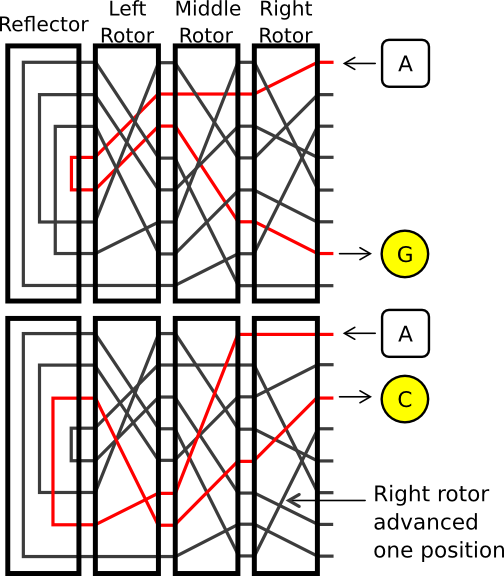
\includegraphics[width=0.5\textwidth,height=0.5\textheight,keepaspectratio]{figures/enigmaaction.png}
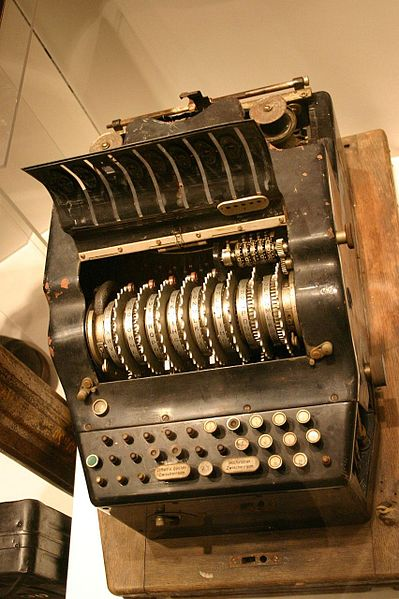
\includegraphics[width=0.5\textwidth,height=0.5\textheight,keepaspectratio]{figures/enigma.jpg}
\caption{Enigma.}
\label{fig-enigma}
\end{figure}
\vspace{-3ex}
\fullcite{cnetenigma,numberphileenigma1,numberphileenigma2}
\end{frame}



\begin{frame}
\frametitle{Princípio de Kerckhoff}
\begin{itemize}
\item Um sistema de criptografia deve ser seguro mesmo se tudo sobre ele for público, exceto a chave.
\item Não confie em segurança por obscuridade.
\end{itemize}
\end{frame}

\begin{frame}
\frametitle{Problemas da criptografia clássica}
\begin{itemize}
\item tornaram-se fracas em face da capacidade computacional dos computadores modernos
\item os métodos eram criados \emph{ad hoc}, sem existir definição e prova de segurança
\item o conhecimento de criptografia estava restrito ao militares e agência de inteligência
\item o número de chaves cresce quadraticamente com o número de participantes (cada comunicação entre pares deve possuir uma chave diferente)
\end{itemize}
\end{frame}

\begin{frame}
\frametitle{Criptografia moderna}
\begin{itemize}
\item padronização das primitivas de criptografia
\item invenção da criptografia de chave pública
\item formalização da definição de segurança
\item aumento da capacidade computacional e internet
\item liberação das restrições de criptografia
\end{itemize}
\end{frame}


\begin{frame}[allowframebreaks]
\frametitle{Diffie-Hellman}
O método proposto por Whitfield Diffie e Martin Hellman permite que duas partes,
que não possuem conhecimento prévio uma da outra, troquem chaves de maneira segura através de um canal público.

\begin{figure}[h]
\centering
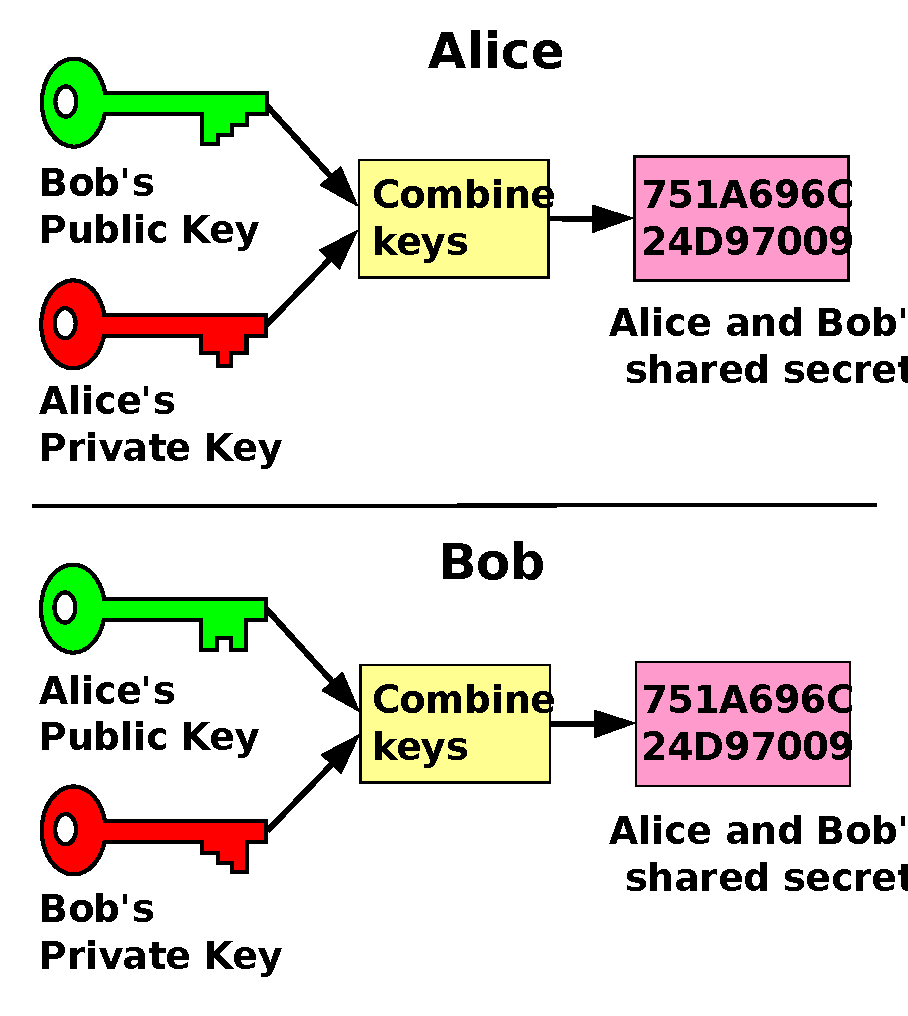
\includegraphics[width=0.6\textwidth,height=0.6\textheight,keepaspectratio]{figures/public_key_shared_secret.pdf}
\caption{Esquema de troca de chaves Diffie-Hellman.}
\label{fig-delffiehellman}
\end{figure}

\framebreak
\begin{itemize}
\item Alice seleciona um grupo $G$ (grupo matemático), um gerador $g$, e um valor aleatório $x$.
\item Alice calcula $A = g^x$ e envia para Bob ($G$,$g$,$A$).
\item Bob seleciona aleatoriamente $y$, calcula $B = g^y$, e envia $B$ para Alice.
\item Alice calcula $K = B^x= g^{(xy)}$.
\item Bob calcula $K = A^y= g^{(xy)}$.
\end{itemize}

$K$ fica sendo a chave que será utilizada na comunicação entre Alice e Bob.

Eve está escutando o canal e obtém ($G$,$g$,$A$,$B$) = ($G$,$g$,$g^x$,$g^y$).

Não existe maneira eficiente de calcular $g^{(xy)}$.

\framebreak
Problemas:
\begin{itemize}
\item ataque \emph{man in the middle}
\item é necessário estabelecer $n^2$ chaves para a comunicação entre $n$ partes ou realizar este protocolo no início de cada comunicação
\item computação sobre alguns grupos pode ser cara
\end{itemize}

\end{frame}


\begin{frame}
\frametitle{Criptografia de chave pública - RSA}
\begin{itemize}
\item par de chaves: pública e privada
\item utiliza-se a chave pública para criptografar uma mensagem
\item apenas a chave privada é capaz de descriptografar
\item RSA (Rivest-Shamir-Adleman) 
\end{itemize}

\end{frame}
